%%%%%%%%%%%%%%%%%%%%%%%%%%%%%%%%%%%%%%%%%%%%%%%%%%%%%%%%%%%%%%%%%%%%%%%%%%%%%%%%%%%%%%%%%%%%%%%%
%
% CS576 Written Question Template
%
% Acknowledgements:
% The original code is written by Prof. James Tompkin (james_tompkin@brown.edu).
% The second version is revised by Prof. Min H. Kim (minhkim@kaist.ac.kr).
%
% This is a LaTeX document. LaTeX is a markup language for producing 
% documents. Your task is to fill out this document, then to compile 
% it into a PDF document. 
%
% 
% TO COMPILE:
% > pdflatex thisfile.tex
%
% If you do not have LaTeX and need a LaTeX distribution:
% - Personal laptops (all common OS): www.latex-project.org/get/
% - We recommend latex compiler miktex (https://miktex.org/) for windows,
%   macTex (http://www.tug.org/mactex/) for macOS users.
%   And TeXstudio(http://www.texstudio.org/) for latex editor.
%   You should install both compiler and editor for editing latex.
%   The another option is Overleaf (https://www.overleaf.com/) which is 
%   an online latex editor.
%
% If you need help with LaTeX, please come to office hours. 
% Or, there is plenty of help online:
% https://en.wikibooks.org/wiki/LaTeX
%
% Good luck!
% Min and the CS576 staff
%
%%%%%%%%%%%%%%%%%%%%%%%%%%%%%%%%%%%%%%%%%%%%%%%%%%%%%%%%%%%%%%%%%%%%%%%%%%%%%%%%%%%%%%%%%%%%%%%%
%
% How to include two graphics on the same line:
% 
% \includegraphics[\width=0.49\linewidth]{yourgraphic1.png}
% \includegraphics[\width=0.49\linewidth]{yourgraphic2.png}
%
% How to include equations:
%
% \begin{equation}
% y = mx+c
% \end{equation}
% 
%%%%%%%%%%%%%%%%%%%%%%%%%%%%%%%%%%%%%%%%%%%%%%%%%%%%%%%%%%%%%%%%%%%%%%%%%%%%%%%%%%%%%%%%%%%%%%%%

\documentclass[11pt]{article}

\usepackage[english]{babel}
\usepackage[utf8]{inputenc}
\usepackage[colorlinks = true,
            linkcolor = blue,
            urlcolor  = blue]{hyperref}
\usepackage[a4paper,margin=1in]{geometry}
\usepackage{stackengine,graphicx}
\usepackage{fancyhdr}
\setlength{\headheight}{15pt}
\usepackage{microtype}
\usepackage{times}
\usepackage{booktabs}

% From https://ctan.org/pkg/matlab-prettifier
\usepackage[numbered,framed]{matlab-prettifier}

\frenchspacing
\setlength{\parindent}{0cm} % Default is 15pt.
\setlength{\parskip}{0.3cm plus1mm minus1mm}

\pagestyle{fancy}
\fancyhf{}
\lhead{Homework Writeup}
\rhead{CS576}
\rfoot{\thepage}

\date{}

\title{\vspace{-1cm}Homework 2 Writeup}


\begin{document}
\maketitle
\vspace{-3cm}
\thispagestyle{fancy}



\section*{Introduction}
\vspace{-5pt}
\subsection*{Scene Recognition with Bag of Words}
\vspace{-5pt}


We performed scene recognition with the bag of words method. We will classify scenes into one of 15 categories by training and testing on the 15 scene database
We implemented three scene recognition schemes:
\vspace{-5pt}
\begin{itemize}
    \item  Build vocabulary by k-means clustering
    \vspace{-5pt}
    \item Principle component analysis(PCA) for vocabulary
    \vspace{-5pt}
    \item Bag of words representation of scenes
    \vspace{-5pt}
    \item Multi-class SVM
\end{itemize}{}
\vspace{-15pt}

\subsection*{Feature-extraction and k-mean clustering to build vocabulary}
\vspace{-5pt}
We used cv2 Python library functions cv2.xfeatures2dSIFT.create() and cv2.HOGDescriptor() to scale-invariant feature transform(SIFT) features and histogram of oriented gradients(HOG) features, respectively. \
We then implemented k-means clustering algorithm that returns k centroids, which have the same dimension as the input data points. We then used these centroids as our vocabulary, so parameter k also means the vocabulary size(the number of words). The algorithm should terminate when the number of iteration reaches a specific maximum, or the difference between the previous centroid and the current centroid is smaller than epsilon for each of k centroids. \

Here is a code snippet for kmeans clustering

    



\vspace{10pt}
\begin{lstlisting}[style=Matlab-editor]
for i in range(vocab_size):
        vocab_matrix[i]= all_features[random_array[i]]
for iteration in range(max_iter):
    dist_mat = pdist(all_features, vocab_matrix)
    c1=0
    for vec in dist_mat:
        index= np.argmin(vec)
        class_arr[c1]= index
        c1 +=1
    sum_in_class = np.zeros((vocab_size, all_features.shape[1]))
    new_vocab_matrix = np.zeros((vocab_size, all_features.shape[1]))
    class_num = np.zeros((vocab_size))
    for i in range(total_pts):
        curr_class = class_arr[i]
        sum_in_class[int(curr_class)] += all_features[i]
        class_num[int(curr_class)] +=1

    for i in range(vocab_size):
        if class_num[i]==0:
            new_vocab_matrix[i]= vocab_matrix[i]
        else:
            new_vocab_matrix[i]= (sum_in_class[i])/ (class_num[i])
    dist_mat1 = pdist(vocab_matrix, new_vocab_matrix)
    for n in range(vocab_size):
        if dist_mat1[n][n] > epsilon:
            break
        if n == vocab_size -1:
            break
    vocab_matrix = new_vocab_matrix
return vocab_matrix

\end{lstlisting}
\subsection*{Principle component analysis(PCA) for vocabulary}
\vspace{-5pt}
By Implemention of PCA on our vocabulary, a set of feature vectors, we reduce the feature dimension to 3. We get the following figure on visualising the PCA result.
 \begin{figure}[h]
    \centering
    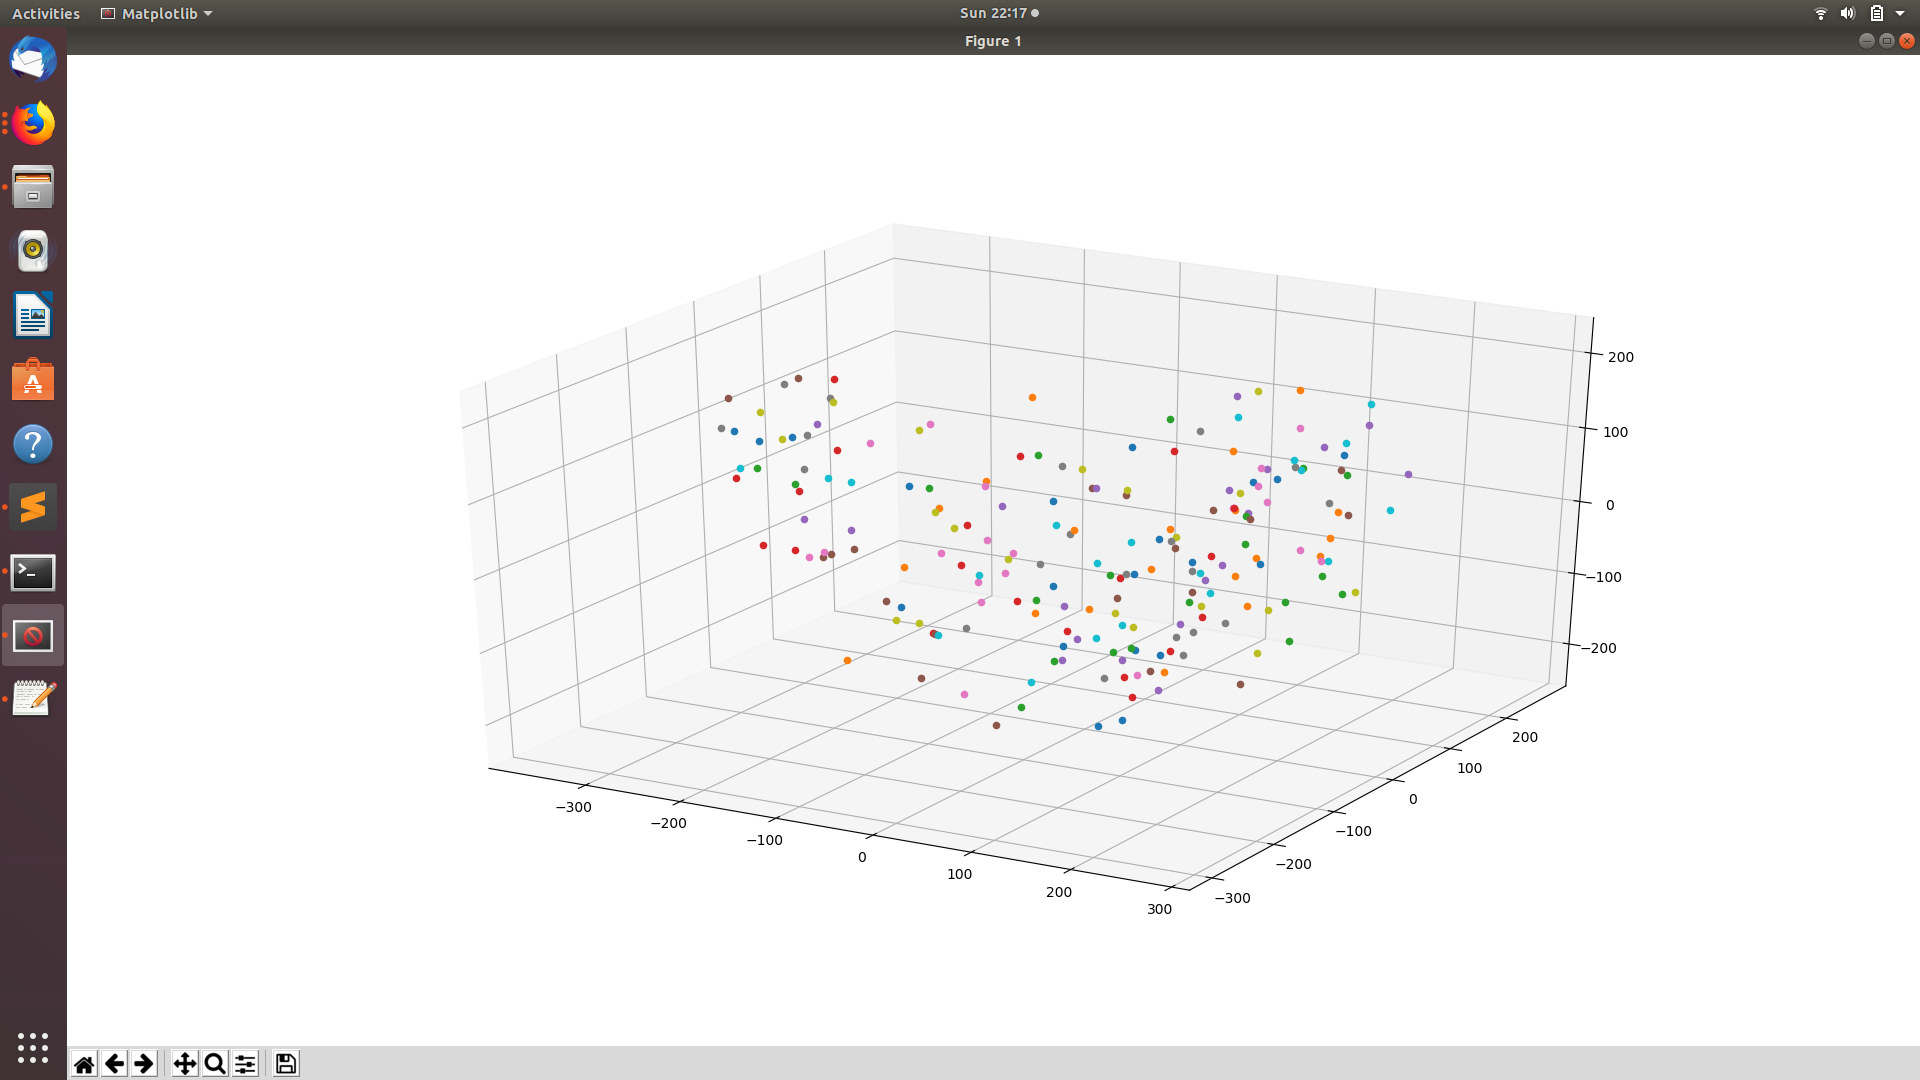
\includegraphics[width=8cm]{img.png}
    \end{figure}

Here is a code snippet for PCA.




\begin{lstlisting}[style=Matlab-editor]
def get_features_from_pca(feat_num, feature):
    if feature == 'HoG':
        vocab = np.load('vocab_hog.npy')
    elif feature == 'SIFT':
        vocab = np.load('vocab_sift.npy')
    mean = np.mean(vocab.T, axis =1)
    centered = vocab -mean
    covar = np.cov(centered.T)
    val, vec = np.linalg.eig(covar)
    l = val.tolist()
    tuple1 = [l.index(x) for x in sorted(l, reverse=True)[:feat_num]]
    ft_size = vocab.shape[1]
    vector1 = np.zeros((ft_size, feat_num))
    for i in range(feat_num):
        vector1[:,i] = vec[:,tuple1[i]]
    final = vector1.T.dot(centered.T)
    print(final)
    return final.T
\end{lstlisting}
\vspace{-10pt}

\subsection*{Bag of words representation of scenes}
\vspace{-5pt}
We now represent our training and testing images as histograms of visual words. This is done by finding the nearest neighbor k-means centroid for every feature descriptor. We then implement the following code to get bag of words representation as a histogram from given image file

Here is a code snippet for the Bag of words representation
\begin{lstlisting}[style=Matlab-editor]
def get_bags_of_words(image_paths, feature):
    if feature == 'HoG':
        vocab = np.load('vocab_hog.npy')
    elif feature == 'SIFT':
        vocab = np.load('vocab_sift.npy')
    vocab_size = vocab.shape[0]
    output_mat = np.zeros((image_paths.shape[0],vocab_size))
    i = 0
    for path in image_paths:
        img = cv2.imread(path)[:, :, :: -1]
        ft = feature_extraction(img, feature)
        distance_mat = pdist(ft, vocab)
        for vec in distance_mat:
            index= np.argmin(vec)
            output_mat[i][index] +=1
        output_mat[i] = output_mat[i] / linalg.norm(output_mat[i])
        i = i+1
    return output_mat
\end{lstlisting}
\vspace{-10pt}

\subsection*{Spatial pyramid representation}
\vspace{-5pt}
One drawback of Bag of Visual Words is, all local features are encoded into a single code vector ignoring the position of the feature descriptors, which means spatial information between words are discarded in the final code vector. Thus, to incorporate the spatial information into the final code vector, one can apply Spatial Pyramid Matching. \\ \\
At a high level, Spatial Pyramid Matching works by breaking up the image into different regions and compute the descriptor and each region, form the histogram of visual words in each region and then concatenate them all into one single 1D vector representation. This somehow incorporates spatial information in our image, thus can capture more features in our image and represent them in histogram form and can also result in a better performance. \\ \\
Say we break the image into L+1 layers (L=0,1,2,...,L) and we assume the length of our codebook is M. At each layer $l$, we break the image into $2^{2l}$ regions (each dimension has $2^l$ cells). For each region, we compute the dense SIFT features and represent them as histogram of visual words just as before. At the end, we concatenate all histogram presentations of image at different levels together to form a long 1D vector. The length of this vector will be $M(\frac{4^{L+1}-1}{3})$. 
The performance improves roughly by 0.02. For C = 0.0004918, our accuracy reported is 0.696.
\begin{lstlisting}[style=Matlab-editor]
x_train = computeSIFT(train_data)
x_test = computeSIFT(test_data)
all_train_desc = []
for i in range(len(x_train)):
    for j in range(x_train[i].shape[0]):
        all_train_desc.append(x_train[i][j,:])
all_train_desc = np.array(all_train_desc)
kmeans = KMeans(n_clusters=k, random_state=0).fit(all_train_desc)
for path in image_paths:
    img = cv2.imread(path)[:, :, ::-1]
    hist = getImageFeaturesSPM(max_level, img, kmeans, k)
    x.append(hist)
return np.array(x)
\end{lstlisting}
\vspace{-15pt}


\subsection*{Multi-class SVM}
\vspace{-5pt}
We finally train 1-vs-all linear SVMs to classify the bag of words feature space. SVM will try to find our linear separable plane using support vectors.  The feature space, the space of the histogram vectors, is partitioned by a learned hyperplane and test cases are categorized based on which side of that hyperplane they fall on.\\\\ Since there are few packages that support multi-class SVM, we can train 15 one-vs-all SVM classifiers for each class and assign the label to the testing image based on the one that gives us the highest response. In other words, we can train 15 SVMs and achieved 15 different hyperparameters called w. For each testing image, its label is assigned based on the label of the classifier that has the highest score (w'x+b).\\ \\When using SVM, we have a hyperparameter C that is tunable, which can yields different performances for the prediction on the testing set. Thus, it's necessary to try different C and report the one that yields the best performance. The accuracy varies from 0.6 to 0.7 depending on the value of C used in the classifier. In our data sample, with C = 0.06148 (roughly) results in the accuracy of 0.6773.\\ \\
Finally, we can evaluate our performance based on the confusion matrix. This matrix consists of all class labels in two dimensions and can be presented in Normalized or Unnormalized form. The Unnormalized form gives us number of correct and incorrect labels for each true class compared to its predicted class. The Normalized form gives us the accuracy (percentage) of our prediction for each class. We evaluate the performance by looking at the diagonal of the matrix, the higher the value along the diagonal, the better of our performance.


\begin{lstlisting}[style=Matlab-editor]
for categ in categories:
    new_train_labels1 = np.zeros((len(train_labels)))
    new_train_labels1 = np.where(train_labels==categ, 1, new_train_labels1)
    classifier = svm.SVC(random_state=0,C=0.025, kernel= kernel_type)
    classifier.fit(train_image_feats, new_train_labels1)
    cfd_arr = classifier.decision_function(test_image_feats)
    cfd_matrix[:,i]= cfd_arr
    i +=1
for vec in cfd_matrix:
    index = np.argmax(vec)
    pred_labels[j]= categories[index]
    j +=1
return pred_labels
\end{lstlisting}
\vspace{-15pt}

\section*{Result}
 When learning an SVM, we have a free parameter $\lambda$ (lambda) which controls how strongly regularized the model is. The accuracy will be very sensitive to $\lambda$.
The results are summarized in the table below.

\begin{table}[h]
    \centering
    \begin{tabular}{lr}
        \toprule
        Condition & Accuracy \\
        \midrule
        linear & 0.725 \\
        rbf & 0.707 \\
        SIFT & 0.725\\
        HoG & 0.691\\
        with spacial pyramid & 0.725\\
        without spacial pyramid & 0.635\\
        
        \bottomrule
    \end{tabular}

\end{table}



\end{document}